\section{\texorpdfstring{Control Web - Procedury}{Control Web - Procedury}}

% =====================================================================================================================
	\begin{frame}
    \frametitle{Procedura}
		\small
		\begin{itemize}
			\item V kontextu CW je to v podstatě téměř totéž co funkce,
			\item může obsahovat parametry a návratovou hodnotu,
			\item může být vázána na přístroj, driver nebo událost,
			\vspace{3mm}
			\item rozlišujeme tři typy:
			
			\begin{itemize}
				\item \textbf{nativní} - zabudované s předem určenou funkcí, 
				\item \textbf{uživatelské} - procedury bez vazby na vnitřní akce systému, volání zajišťuje aplikace,
				\item \textcolor{blue}{\textbf{událostní}} - procedury s vazbou na akci systému.
			\end{itemize}
		\end{itemize}

	\end{frame}
	
% =====================================================================================================================
	\begin{frame}
    \frametitle{Událostní procedury}
		
		\begin{minipage}[t][\textheight][t]{0.55\textwidth}
		\small
		\textbf{Inspektor:}
		
			\begin{center}
				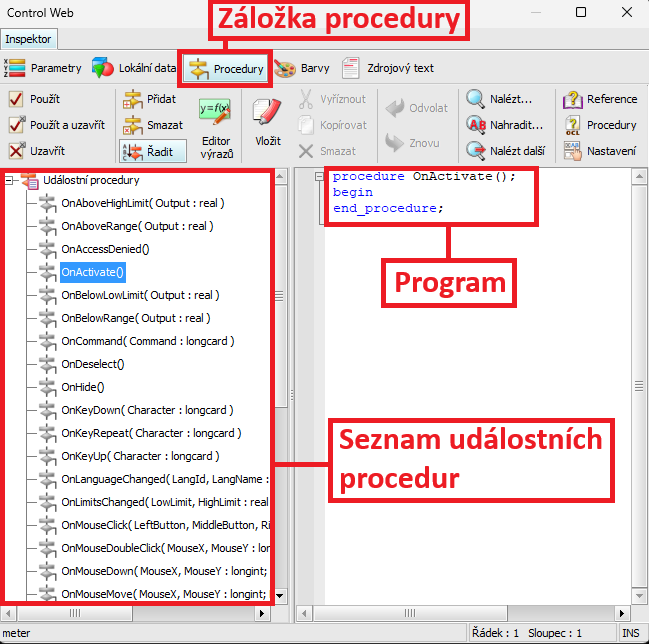
\includegraphics[width=1\textwidth]{fig/inspektor_procedury.png}
			\end{center}

		\end{minipage}
		\begin{minipage}[t][\textheight][t]{0.4\textwidth}
		
			\small
			\begin{itemize}
				\item Pro příklad je použita stejná APP jako při ovladačích,
				\item různé typy podle vazby:
				
				\begin{itemize}
					\item \textcolor{blue}{\textbf{OnActivate()}},
					\item OnHide(),
					\item OnMouseClick(),
				\end{itemize}
				
				\item program v jazyce OCL
			\end{itemize}
			
			Procedura \textcolor{blue}{\textbf{OnActivate()}} je volána při každé aktivaci přístroje - například periodou časování.
		\end{minipage}

	\end{frame}
	
% =====================================================================================================================
	\begin{frame}
    \frametitle{OCL (Object Control Language)}
		
		\begin{itemize}
			\item Je skriptovací jazyk pro psaní procedur a programu,
			\item jazyk je specifický pro CW.
		\end{itemize}
		
		\begin{minipage}[t][\textheight][t]{0.55\textwidth}
		\small
		\textbf{Textový editor:}
		
			\begin{center}
				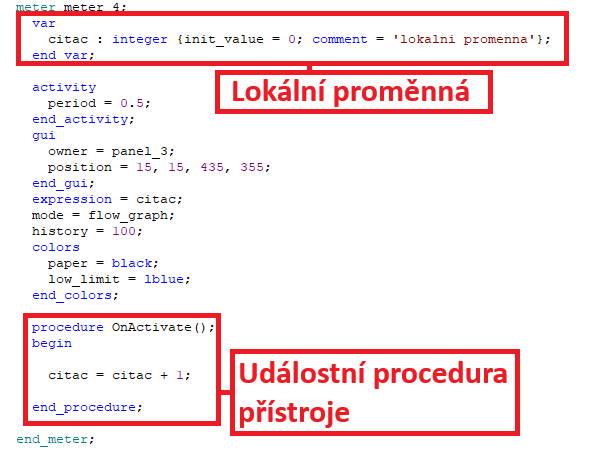
\includegraphics[width=1\textwidth]{fig/ocl_prirazeni.png}
			\end{center}

		\end{minipage}
		\begin{minipage}[t][\textheight][t]{0.4\textwidth}
		
			\small
			\begin{itemize}
				\item Proměnné
				
				\begin{itemize}
					\item lokální - deklarace přístroji,
					\item globální - deklarace v datovém editoru
				\end{itemize}
				\item Přiřazujeme pomocí =,
				\item lze používat všechny obvyklé operátory: +, -, \&, and, ...
				\item řádky zakončujeme středníkem.
				
			\end{itemize}
			
		\end{minipage}

	\end{frame}
	
% =====================================================================================================================
	\begin{frame}
    \frametitle{Podmíněné větvení pomocí \textbf{if}}
		
		\textbf{POZOR:} \uv{\textcolor{red}{\textbf{citac}}} je globalní proměnná, lokální se vytváří znovu při každém volání procedury.
		
		\begin{minipage}[t][\textheight][t]{0.55\textwidth}
		\small
		\textbf{APP:}
		
			\begin{center}
				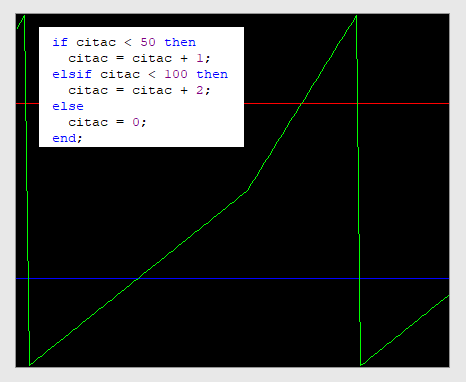
\includegraphics[width=1\textwidth]{fig/ocl_podminka.png}
			\end{center}

		\end{minipage}
		\begin{minipage}[t][\textheight][t]{0.4\textwidth}
		
			\small
			\begin{itemize}
				\item Vyhodnocován je Booleovský stav,
				\item pro relace používáme: $>$, $<$, $>$$=$, ...
				\item \textcolor{red}{\textbf{příkazy jsou malými písmeny}},
				\item po \textcolor{blue}{\textbf{if}} a \textcolor{blue}{\textbf{elsif}} následuje \textcolor{blue}{\textbf{then}},
				\item větvení končí příkazem \textcolor{blue}{\textbf{end}} se středníkem.
				
			\end{itemize}
			
		\end{minipage}

	\end{frame}
	
% =====================================================================================================================
	\begin{frame}
    \frametitle{Podmíněné větvení pomocí \textbf{switch}}
		
		\begin{minipage}[t][\textheight][t]{0.55\textwidth}
		\small
		\textbf{APP:}
		
			\begin{center}
				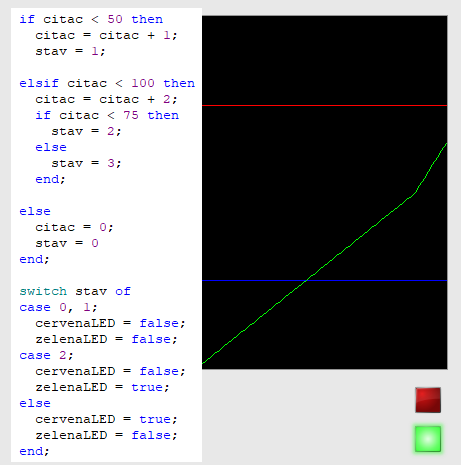
\includegraphics[width=1\textwidth]{fig/ocl_switch.png}
			\end{center}

		\end{minipage}
		\begin{minipage}[t][\textheight][t]{0.4\textwidth}
		
			\small
			\begin{itemize}
				\item Vyhodnocována je celá hodnota,
				\item pod jeden \textcolor{blue}{\textbf{case}} lze psát více hodnot oddělených čárkou,
				\item větvení končí příkazem \textcolor{blue}{\textbf{end}} se středníkem.
				
			\end{itemize}
			
		\end{minipage}

	\end{frame}
	
% =====================================================================================================================
	\begin{frame}
    \frametitle{Další příkazy OCL}
		
		\small
		Po stisku \textbf{F1} a vyhledání \uv{\textcolor{blue}{\textbf{Programování a procedury — OCL}}}:
		
		
		\begin{itemize}
			\item Psaní uživatelských procedur, přidávání návratových hodnot,
			\item návěstí a příkaz \textcolor{blue}{\textbf{goto}},
			\item cykly:
			
			\begin{itemize}
				\item \textcolor{blue}{\textbf{loop}} - nekonečná smyčka,
				\item \textcolor{blue}{\textbf{while}} - smyčka s testem podmínky na začátku,
				\item \textcolor{blue}{\textbf{repeat until}} - smyčka s testem podmínky na konci,
				\item \textcolor{blue}{\textbf{for}} - smyčka s počítadlem,
			\end{itemize}
			
			\item zdržení programu:
			
			\begin{itemize}
				\item \textcolor{blue}{\textbf{pause}} - uspání jen v rámci dané funkce,
				\item \textcolor{blue}{\textbf{wait}} - zastavení běhu programu,
			\end{itemize}
			
			\item aktivace přístrojů \textcolor{blue}{\textbf{send}},
			\item návrat z procedury \textcolor{blue}{\textbf{return}}, ...
			
		\end{itemize}

	\end{frame}